\chapter{Supplemental Information}

\section*{Histogram}
\begin{figure}[h!]
	\centering
	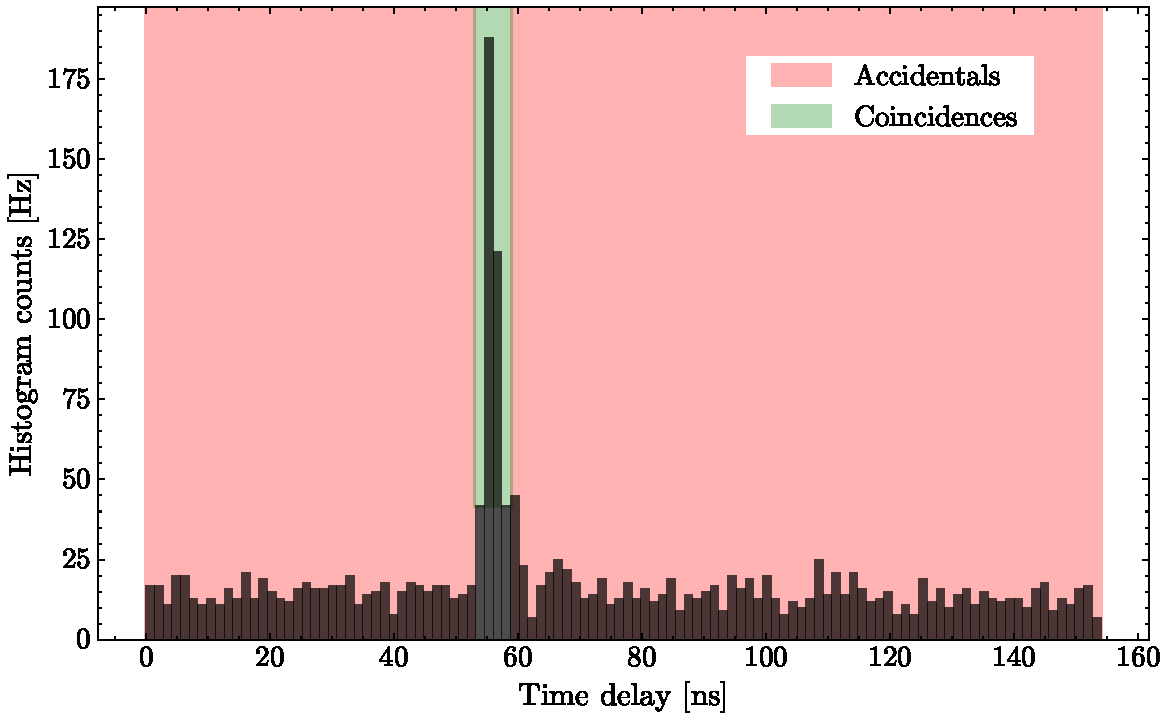
\includegraphics[width=.7\textwidth]{Images/HistogramExample.pdf}
	\caption{Representative coincidence histogram using the experimental setup}
	\label{fig:HistExamAcc}
\end{figure}

\section*{Afterpulsing}
\begin{figure}[h!]
	\centering
	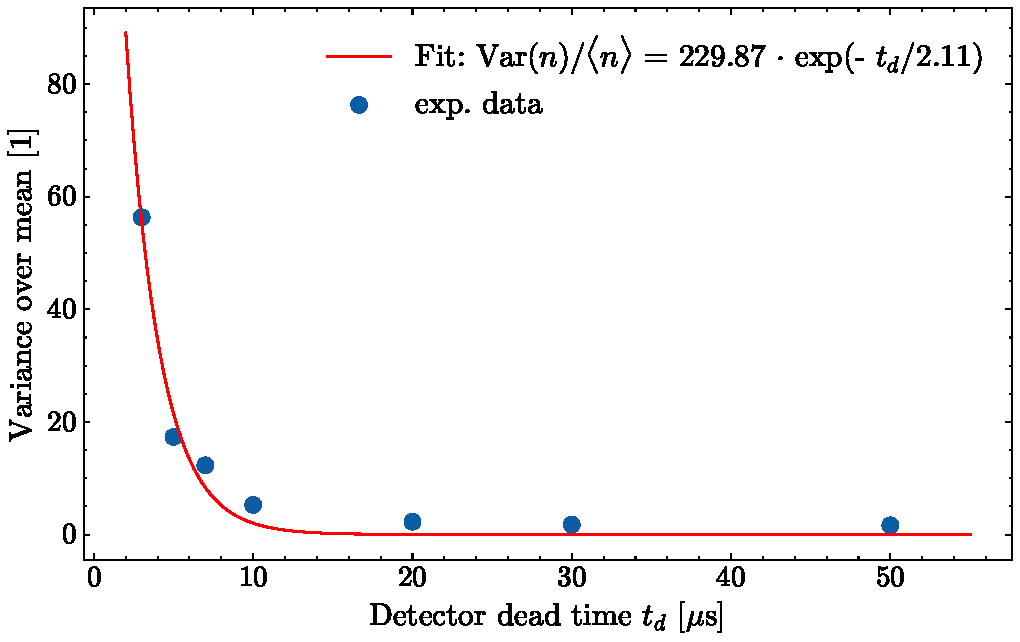
\includegraphics[width=.7\textwidth]{Images/VarMean_DeadTime_Afterpulsing.pdf}
	\caption{Variance-to-mean ratio as a function of the dead time of the IR single-photon detector}
	\label{fig:VoMDead}
\end{figure}
\newpage
\section*{Dark counts SNSPD}
\begin{figure}[h!]
	\centering
	% First figure
	\begin{minipage}[t]{\textwidth}
		\centering
		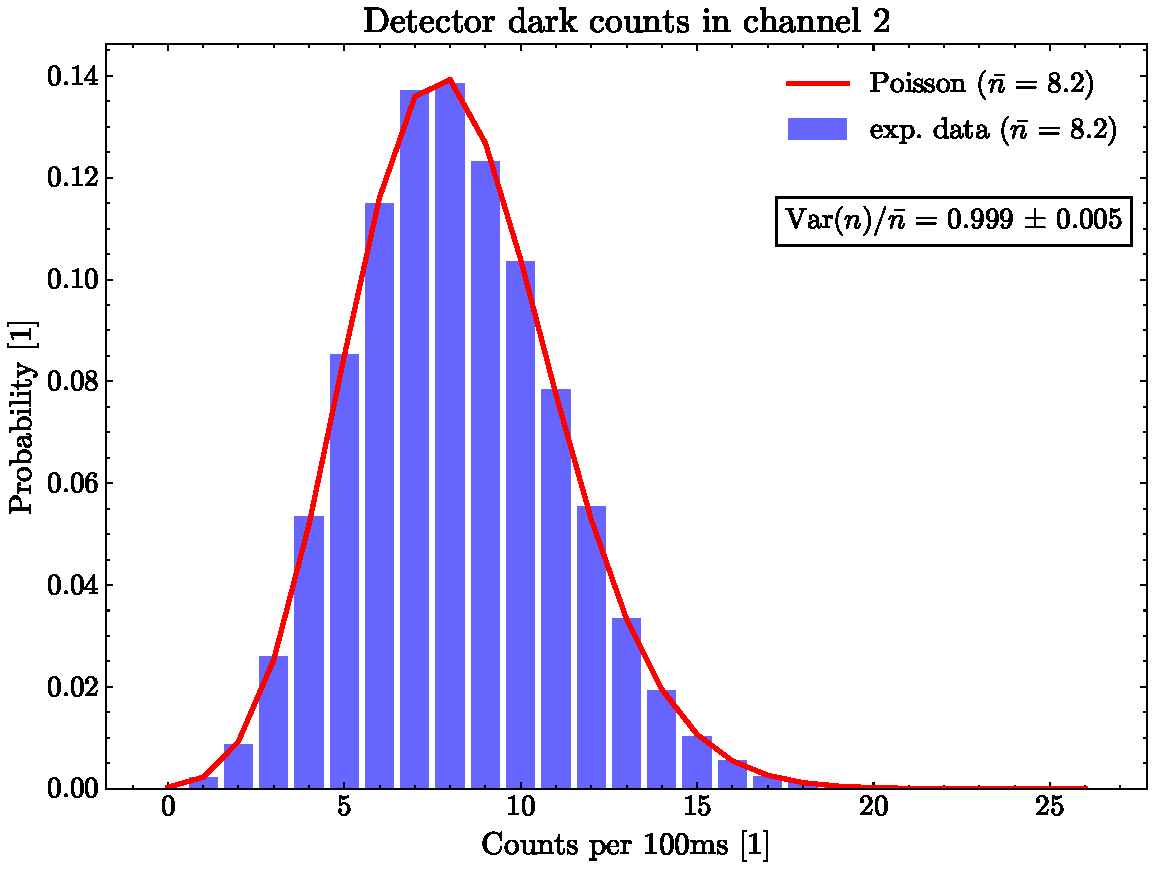
\includegraphics[page=1,width=.8\linewidth]{Images/DC_chAll.pdf}
		%\caption{Caption for Figure 1}
	\end{minipage}
	
	%\vspace{1cm} % space between figures
	
	% Second figure
	\begin{minipage}[t]{\textwidth}
		\centering
		\includegraphics[page=2,width=.8\linewidth]{Images/DC_chAll.pdf}
		%\caption{Caption for Figure 2}
	\end{minipage}
	
	%\vspace{1cm}
	
	% Third figure
	\begin{minipage}[t]{\textwidth}
		\centering
		\includegraphics[page=3,width=.8\linewidth]{Images/DC_chAll.pdf}
		%\caption{Caption for Figure 3}
	\end{minipage}
	\caption{Dark counts of the SNSPD}
	\label{fig:DC}
\end{figure}


%\begin{figure}[h!]
%	\noindent
%	\begin{minipage}{0.33\textwidth}
%		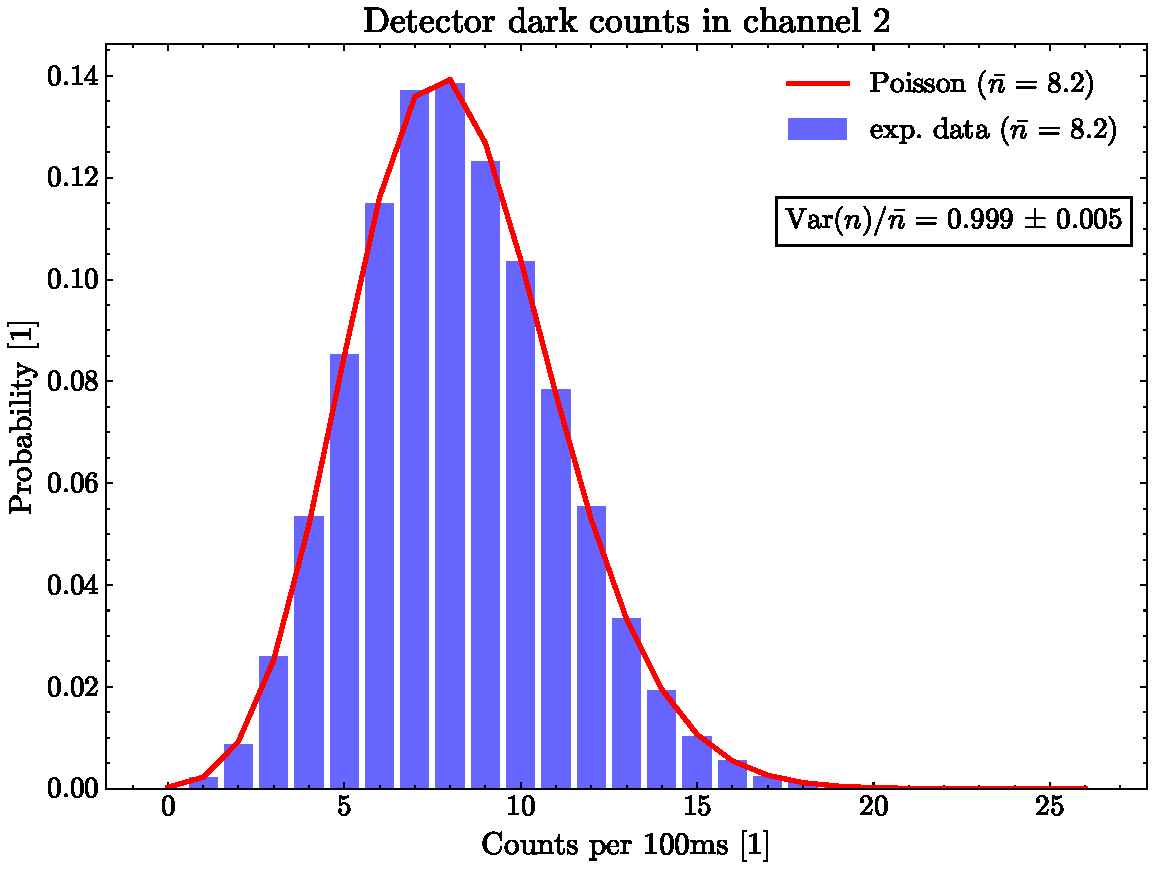
\includegraphics[page=1,width=\linewidth]{Images/DC_chAll.pdf}
%	\end{minipage}%
%	\begin{minipage}{0.33\textwidth}
%		\includegraphics[page=2,width=\linewidth]{Images/DC_chAll.pdf}
%	\end{minipage}%
%	\begin{minipage}{0.33\textwidth}
%		\includegraphics[page=3,width=\linewidth]{Images/DC_chAll.pdf}
%	\end{minipage}
%	\caption{Dark counts of the SNSPD}
%	\label{fig:DC}
%\end{figure}



